%%%%%%%%%%%%%%%%%%%%%%%%%%%%%%%%%%%%%%%%%%%%%%%%%%%%%%%%%%%%%%%%%%%%%%%%%%%%%%%%%%%%%
%                        Author: Harshit Prashant Dhanwalkar                        %
%%%%%%%%%%%%%%%%%%%%%%%%%%%%%%%%%%%%%%%%%%%%%%%%%%%%%%%%%%%%%%%%%%%%%%%%%%%%%%%%%%%%%

%-------------------------------------------------------------------------------------
%                    PACKAGES AND OTHER DOCUMENT CONFIGURATIONS                      %
%-------------------------------------------------------------------------------------
\documentclass[fleqn,10pt]{SelfArx} % Document font size and equations flushed left
\usepackage[english]{babel} 
\usepackage{enumitem}

\usepackage{tikz}
\usetikzlibrary{trees, positioning}
\usetikzlibrary{shapes, shadings}
\usepackage{tikz-3dplot}
\usetikzlibrary{3d,shapes.geometric,shadows.blur}
\tikzstyle{vertex}=[draw,fill=black!15,circle,minimum size=20pt,inner sep=0pt]
\tikzstyle{selected edge} = [draw,line width=5pt,-,red!50]

\usepackage{amsmath}
\usepackage{array} % for tables

% \usepackage[table,xcdraw]{xcolor}
% \usepackage[table, dvipsnames]{xcolor}

\usepackage{pgfplots}
\pgfplotsset{compat=1.18}
\tdplotsetmaincoords{60}{115}
\pgfplotsset{compat=newest}

\usepackage{subfig}

%-------------------------------------------------------------------------------------
%                                       COLUMNS                                      %
%-------------------------------------------------------------------------------------
\setlength{\columnsep}{0.55cm} % Distance between the two columns of text
\setlength{\fboxrule}{0.75pt} % Width of the border around the abstract

%-------------------------------------------------------------------------------------
%                                       EQUATIONS                                    %
%-------------------------------------------------------------------------------------
\usepackage{cancel} % for crossing the word showing it is cancelled or is zero

%-------------------------------------------------------------------------------------
%                                     EQUATIONLINKS                                  %
%-------------------------------------------------------------------------------------
\newcommand{\myeqref}[1]{Eq.\textcolor{blue}{\textup{(\getrefnumber{#1})}}}

%-------------------------------------------------------------------------------------
%                                        COLORS                                      %
%-------------------------------------------------------------------------------------
\definecolor{color1}{RGB}{0,0,90} % Color of the article title and sections
\definecolor{color2}{RGB}{0,20,20} % Color of the boxes behind the abstract and headings

%-------------------------------------------------------------------------------------
%                                       HYPERLINKS                                   %
%-------------------------------------------------------------------------------------
\usepackage{xcolor}
\usepackage{hyperref}
\usepackage{footnote}

%\newcommand{\myhref}[2]{\href{#1}{\textcolor{blue}{#2}}}
\newcommand{\myhref}[2]{%
  \href{#1}{\textcolor{blue}{#2}}%
  \footnote{\url{#1}}%
}

\usepackage{cleveref}
% Customize cleveref to use "Eq." for equations
\crefname{equation}{Eq.}{Eq.}
\Crefname{equation}{Eq.}{Eq.}

\hypersetup{
	hidelinks,
	colorlinks,
	breaklinks=true,
	urlcolor=color2,
	citecolor=blue!90,
	linkcolor=color1,
	bookmarksopen=false,
	pdftitle={Title},
	pdfauthor={Author},
}

% ------------------------------------------------------------------------------------
%                                       CUSTOM  SYMBOLS                              %
%-------------------------------------------------------------------------------------
\newcommand{\zbar}{\raisebox{0.2ex}{--}\kern-0.6em Z}

% ------------------------------------------------------------------------------------
%                                       CUSTOM  YELLOW STICKY NOTES		     %
%-------------------------------------------------------------------------------------
\usepackage{color, colortbl}
\usepackage{calc}

\setlength{\parskip}{0ex}
\setlength{\parindent}{0ex}

\newlength{\yellownotewidth}
\setlength{\yellownotewidth}{2.5cm}
\newlength{\yellownoteheight}
\setlength{\yellownoteheight}{2cm}

% Yellow note...
\newcommand{\yellownote}[1]{
    \vspace{0.2\yellownoteheight}
        \begin{center}
        \begin{tikzpicture}
            % Shadow effect
            \draw[white,fill=gray!70,opacity=0.75,shift={(-0.15,-0.15)}]
		    (0,0) -- (0.07, \yellownoteheight) -- (\yellownotewidth + 0.05, \yellownoteheight) -- (2.5, 0.4) -- (2.2,0.18) -- (2, 0) -- cycle;
            % Yellow note background
	    \draw[fill=yellow!35]
		    (0,0) -- (0, \yellownoteheight) -- (\yellownotewidth, \yellownoteheight) -- (2.5, 0.4) -- (2.1,0.2) -- (1.7, 0) -- cycle;
            % Folded corner
            \draw[opacity=0.45,fill=gray!50] (0.7\yellownotewidth,0) -- 
                (0.9\yellownotewidth,0.45) -- (\yellownotewidth,0.4) -- cycle;
            % Note content
            \node[blue,below] at (0.5\yellownotewidth,\yellownoteheight) {
                \begin{minipage}{\yellownotewidth-1em}
                    \scriptsize\sf#1
                \end{minipage}
            };
        \end{tikzpicture}
        \end{center}
}

% Floating yellow note
\newcommand{\freeyellownote}[3]{
    \begin{tikzpicture}[remember picture,overlay]
        \node[anchor=north west, xshift=#1, yshift=#2] at (current page.north west) {
            \begin{tikzpicture}
            % Shadow effect
            \draw[white,fill=gray!70,opacity=0.75,shift={(-0.15,-0.15)}]
		    (0,0) -- (0.07, \yellownoteheight) -- (\yellownotewidth + 0.05, \yellownoteheight) -- (2.5, 0.4) -- (2.2,0.18) -- (2, 0) -- cycle;
            % Yellow note background
	    \draw[fill=yellow!35]
		    (0,0) -- (0, \yellownoteheight) -- (\yellownotewidth, \yellownoteheight) -- (2.5, 0.4) -- (2.1,0.2) -- (1.7, 0) -- cycle;
                % Folded corner
                \draw[opacity=0.45,fill=gray!50] 
                    (0.7\yellownotewidth,0) -- 
                    (0.9\yellownotewidth,0.45) -- 
                    (\yellownotewidth,0.4) -- 
                    cycle;
                % Note content
                \node[blue,below] at (0.5\yellownotewidth,\yellownoteheight) {
                    \begin{minipage}{\yellownotewidth-1em}
                        \scriptsize\sf#3
                    \end{minipage}
                };
            \end{tikzpicture}
        };
    \end{tikzpicture}
}

\definecolor{LightCyan}{rgb}{0.88,1,1}
%-------------------------------------------------------------------------------------
%                                       ARTICLE INFORMATION                          %
%-------------------------------------------------------------------------------------
\JournalInfo{Dual Degree Engineering Physics, 8$^{th}$ Semester, 2024} % Journal information
\Archive{Mtech, Earth System Sciences (ESS), 1$^{st}$ year} % Additional notes (e.g. copyright, DOI, review/research article)

\PaperTitle{Lecture Notes on Boundary Layer Meteorology} % Article title

\Authors{Harshit Prashant Dhanwalkar (SC21B164)\textsuperscript{1}*} % Authors
\affiliation{\textsuperscript{1}\textit{MTech, Earth System Sciences (ESS), 1$^{st}$ year, Department of Physics, Indian Institute Of Spacescience and Technology (IIST)}} % Author affiliation
\affiliation{*\textbf{email}: harshitpd1729@gamil.com} % Corresponding author

\Keywords{} % Keywords - if you don't want any simply remove all the text between the curly brackets
\newcommand{\keywordname}{Keywords} % Defines the keywords heading name

%-------------------------------------------------------------------------------------
%                                           ABSTRACT                                 %
%-------------------------------------------------------------------------------------
\Abstract{Notes of Lectures and addional information from books: \\ \textit{An introduction to boundary layer meteorology}(\cite{stull1988introduction}).}

%-------------------------------------------------------------------------------------
%                                            DOCUMENT                                %
%-------------------------------------------------------------------------------------
\begin{document}
\maketitle % Output the title and abstract box
\thispagestyle{empty} % Removes page numbering from the first page
\clearpage

\begingroup
\thispagestyle{empty} % No page number
\tableofcontents
\endgroup
\newpage

\begingroup
\thispagestyle{empty} % No page number
\listoffigures
\endgroup
\newpage
%-------------------------------------------------------------------------------------
%                                       DOCUMENT CONTENTS                           %
%-------------------------------------------------------------------------------------
%\addcontentsline{toc}{section}{Introduction} % Adds this section to the table of contents
%-------------------------------------------------------------------------------------
\section{Lecture 1 09/01/2025}
\subsection{Introduction To Boundary Layer}
The Boundary Layer can be defined as part of  the troposphere that is directly influenced by the presence of the Earth's surface and responds to surface forcings with a time scale of about an hour or less.

\begin{figure}[ht!]
	\centering
	\resizebox{0.35\textwidth}{!}{
		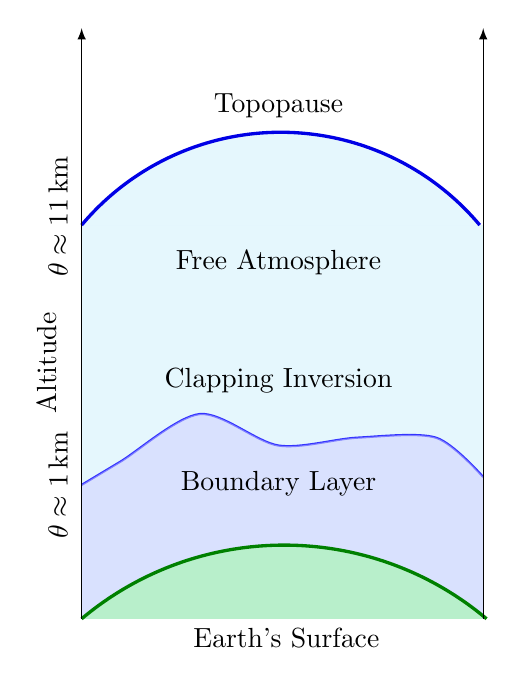
\begin{tikzpicture}
			%Free Atmosphere curve
			\fill[cyan!20, opacity=0.5] (-0.5,0) rectangle (4.6,5);
			\fill[cyan!20, opacity=0.5]
			(-0.5,5) arc[start angle=140, end angle=40, radius=3.3cm] -- (4.6,5) -- cycle;
			\draw[very thick, blue!90!black]
			(-0.5,5) arc[start angle=140, end angle=40, radius=3.3cm];
			\node[anchor=north] at (2,4.8) {Free Atmosphere};
			%Topopause curve
			\node[anchor=north] at (2,6.8) {Topopause};
			%Clapping Inversion curve
			\draw[thick,blue!80] plot [smooth] coordinates {(-0.5, 1.7) (0,2) (1,2.6) (2,2.2) (3,2.3) (4,2.3) (4.6,1.8)};
			\fill[blue!20,opacity=0.5] (-0.5,0) -- plot [smooth] coordinates {(-0.5, 1.7) (0,2) (1,2.6) (2,2.2) (3,2.3) (4,2.3) (4.6,1.8)}  -- (4.6,0) -- cycle;
			\node[anchor=north] at (2,3.3) {Clapping Inversion};
			% Boundary layer curve
			\node[anchor=north] at (2,2) {Boundary Layer};
			% Earth's surface
			\fill[green!40,opacity=0.5]
			(2.5-3,0) arc[start angle=130, end angle=50, radius=4cm] -- (2.5,0) -- cycle;
			\draw[very thick, green!50!black, shift={(2.5,0)}]
			(-3,0) arc[start angle=130, end angle=50, radius=4cm];
			\node[below] at (2.1,0) {Earth's Surface};
			% Axis label
			\draw[-latex] (-0.5,0) -- (-0.5,7.5);
			\node[above, rotate=90] at (-0.7,3.25) {Altitude};
			\draw[-latex] (4.6,0) -- (4.6,7.5);
			% Labels
			\node[anchor=east, rotate=90] at (-0.8,6) {\(\theta \approx 11 \, \mathrm{km}\)};
			\node[anchor=east, rotate=90] at (-0.8,2.5) {\(\theta \approx 1 \, \mathrm{km}\)};
		\end{tikzpicture}
	}
	\renewcommand{\thefigure}{1.1}
	\caption{Atmosphere can be divided into 2 parts: boundary layer near surface and free atmosphere above it.}
\end{figure}

\subsection{Boundary Layer Forcing Mechanism}
What physical process modify boundary layer air parcel?
\begin{enumerate}[noitemsep]
	\item Heat transfer to.from the ground.
	\item Frictional drag.
	\item Evaporation/transpiration.
	\item Terrain-induced flow modification.
	\item Pollution emission.
\end{enumerate}

\subsection{Types Of Air Flow Or Wind}
Air flow or wind can be decomposed into following 3 types:
\begin{enumerate}[noitemsep]
	\item \textbf{Mean Wind} $(\bar{u}, \bar{v}, \bar{w})$: Represents the average wind components in the horizontal ($\bar{u}, \bar{v}$) and vertical ($\bar{w}$) directions. It is important for the horizontal transport of quantities such as moisture, heat, momentum, and pollutants, a process known as advection.
	\item \textbf{Waves}: Atmospheric waves, such as gravity waves, occur mostly at night in the nocturnal boundary layer (NBL). They can influence the structure of the boundary layer and the transport of energy.
	\item \textbf{Turbulence}: The vertical transport of moisture, heat, momentum, and pollutants is primarily dominated by turbulence, which is characterized by chaotic and irregular motion.
\end{enumerate}

\begin{figure}[ht!]
	\centering
	\resizebox{0.45\textwidth}{!}{
		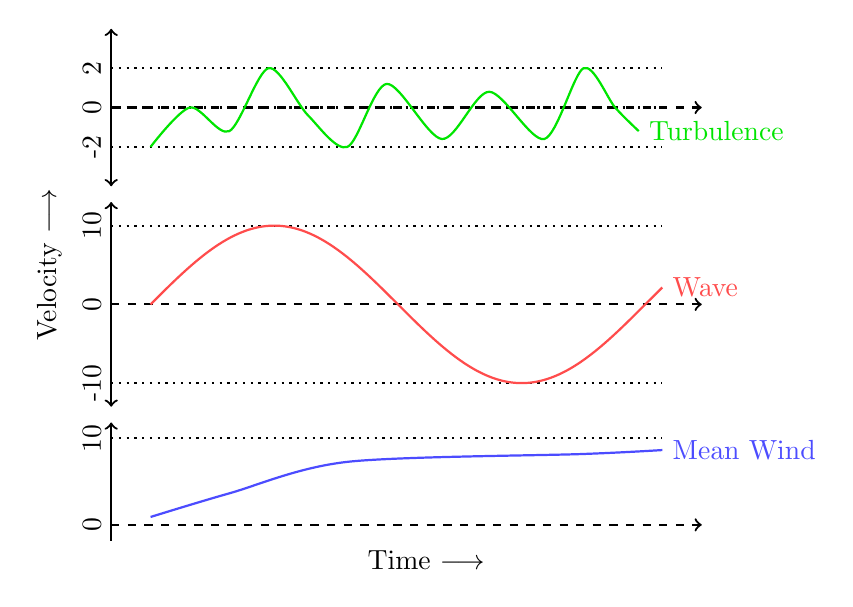
\begin{tikzpicture}[smooth, thick]
			% Axes
			\draw[->] (0,0.5) -- (0,2);
			\draw[<->] (0,2.2) -- (0,4.8);
			\draw[<->] (0,5) -- (0,7);
			\node[above, rotate=90] at (-0.5,4) {Velocity $\longrightarrow$};
			\draw[dashed,->] (0,0.7) -- (7.5,0.7);
			\node[above, rotate=90] at (0,0.7) {0};
			\draw[dashed,->] (0,3.5) -- (7.5,3.5);
			\node[above, rotate=90] at (0,3.5) {0};
			\draw[dashed,->] (0,6) -- (7.5,6);
			\node[below] at (4,0.5) {Time $\longrightarrow$};
			% dottted lines
			%mean
			\draw[dotted, thick] (0,1.8) -- (7,1.8);
			\node[above, rotate=90] at (0,1.8) {10};
			% wave
			\draw[dotted, thick] (0,4.5) -- (7,4.5);
			\node[above, rotate=90] at (0,4.5) {10};
			\draw[dotted, thick] (0,2.5) -- (7,2.5);
			\node[above, rotate=90] at (0,2.5) {-10};
			%tur
			\draw[dotted, thick] (0,5.5) -- (7,5.5);
			\node[above, rotate=90] at (0,5.5) {-2};
			\draw[dotted, thick] (0,6) -- (7,6);
			\node[above, rotate=90] at (0,6) {0};
			\draw[dotted, thick] (0,6.5) -- (7,6.5);
			\node[above, rotate=90] at (0,6.5) {2};
			% Mean Wind (Offset by +2 for vertical distance)
			\draw[blue!70] plot coordinates {(0.5,0.8) (1.5,1.1) (3,1.5) (6,1.6) (7,1.65)}
			node[anchor=west] {Mean Wind};
			% Wave (Sine curve, offset by +4)
			\draw[red!70] plot[domain=0.5:7,samples=100]
			({\x},{3.5 + sin((\x - 0.5) r)})
			node[anchor=west] {Wave};
			% Turbulence (Offset by +6)
			\draw[green!90!black] plot coordinates {(0.5,5.5) (1,6) (1.5,5.7) (2,6.5) (2.5,5.9) (3,5.5) (3.5,6.3) (4.2,5.6) (4.8,6.2) (5.5,5.6) (6,6.5) (6.4,6) (6.7,5.7)}
			node[anchor=west] {Turbulence};
		\end{tikzpicture}
	}
	\renewcommand{\thefigure}{1.2}
	\caption{Plot showing profiles of Mean, Wave and Turbulent winds}
\end{figure}

\subsection{Eddies}
Eddies are formed due to the interaction of currents with obstacles like coastlines, underwater topography, or other currents, as well as from the instability of larger current systems.
Eddies exhibit a rotational flow pattern, either clockwise or counterclockwise.
Eddies can vary from size 100 to 3000 metres and also can exists as small as few millimetres.
Small eddies might last for seconds to minutes, while larger oceanic eddies can persist for weeks, months, or even years.

\subsection{Turbulence Generation Mechanisms}
\begin{itemize} [noitemsep]
	\item \textbf{Solar Heating}: Solar heating generates thermals, which are essentially larger eddies that drive turbulence in the atmospheric boundary layer.
	\item \textbf{Wind Shear}: Variations in wind speed or direction with height create wind shear, which is a significant source of turbulence.
	\item \textbf{Obstacle-Induced Flow}: Deflected flow around obstacles such as trees, buildings, or other structures generates turbulent eddies downstream of these obstacles, creating turbulent wakes.
\end{itemize}

\begin{figure}[ht!]
	\centering
	\resizebox{0.45\textwidth}{!}{
		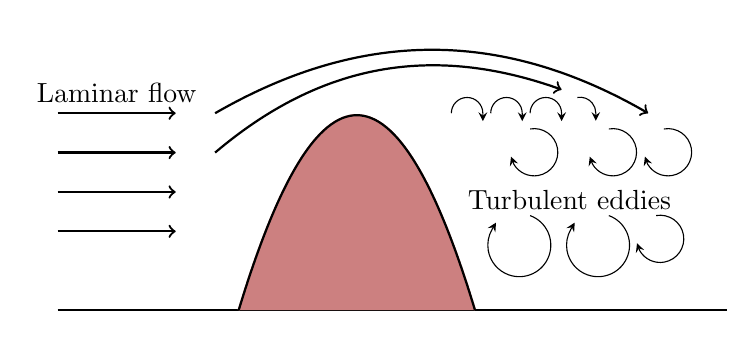
\begin{tikzpicture}
			% Ground
			\draw[thick] (-1,0) -- (7.5,0);
			% Obstacle
			\filldraw[thick, red!60!black!50] (1.3,0) .. controls (2.3,3.3) and (3.3,3.3) .. (4.3,0);
			\draw[thick]  (1.3,0) .. controls (2.3,3.3) and (3.3,3.3) .. (4.3,0);
			% Laminar flow arrows
			\draw[->,thick] (-1,2.5) -- (0.5,2.5) node[midway,above] {Laminar flow};
			\draw[->,thick] (-1,2) -- (0.5,2);
			\draw[->,thick] (-1,1.5) -- (0.5,1.5);
			\draw[->,thick] (-1,1) -- (0.5,1);
			% b/w laminar and eddies
			\draw[->,thick] (1,2) to[bend left] (5.4,2.8);
			\draw[->,thick] (1,2.5) to[bend left] (6.5,2.5);
			% Turbulent eddies
			\foreach \x in {4, 4.5, 5}
			\draw [>=stealth,->] (\x,2.5) arc (180:0:.2cm) -- +(270:0.1cm);
			\draw [>=stealth,->] (5.6,2.7) arc (100:0:.2cm) -- +(270:0.1cm);
			\foreach \x in {5, 6, 6.7}
			\draw [>=stealth,->] (\x,2.3) arc (100:-150:.3cm) -- +(110:0.1cm);
			\draw [>=stealth,->] (6.6,1.2) arc (100:-150:.3cm) -- +(110:0.1cm);
			\foreach \x in {5,6}
			\draw [>=stealth,->] (\x,1.2) arc (70:-210:.4cm) -- +(60:0.1cm);
			\node at (5.5,1.4) {Turbulent eddies};
		\end{tikzpicture}
	}
	\renewcommand{\thefigure}{1.3}
	\caption{Eddy formation due to Turbulence caused by an obstacle}
\end{figure}

Large eddies will break into smaller eddies after which small eddies dissipates from K.E. to thermal energy.

\begin{figure}[ht]
	\centering
	\resizebox{0.45\textwidth}{!}{
		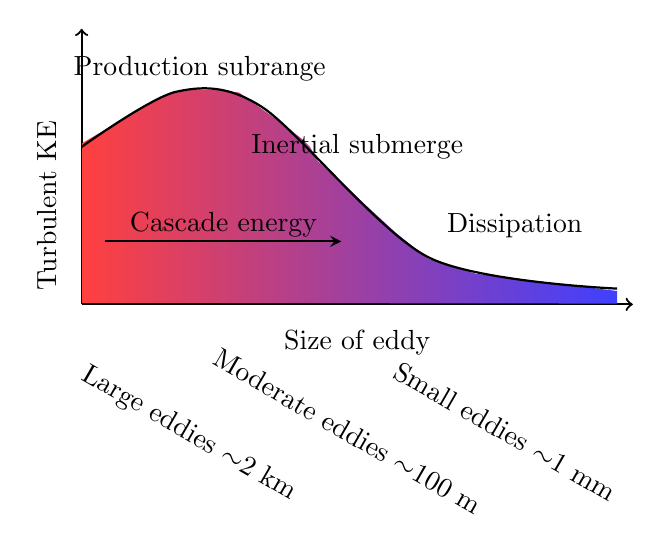
\begin{tikzpicture}
			% Axes
			\draw[thick,->] (0,0) -- (7,0);
			\node[below] at (3.5,-0.2) {Size of eddy};
			\draw[thick,->] (0,0) -- (0,3.5);
			\node[above, rotate=90] at (-0.2,1.25) {Turbulent KE};
			% Curve
			%\filldraw[blue!50, thick, smooth](0.03,0.04) -- plot coordinates {(0.03,2) (1.2,2.7) (2.3,2.5) (4.4,0.6) (6.8,0.2)} -- (6.8,0.04) -- cycle;
			\shade[left color=red!75, right color=blue!75] (0.01,0.02) -- plot coordinates {(0.01,2.05) (1,2.625) (1.25, 2.71) (1.5,2.73) (1.75,2.72) (2,2.69) (2.5,2.33) (2.8,2.1) (2.9,2) (3,1.82) (4,0.9) (4.4,0.58) (5,0.39) (6.8,0.17)} -- (6.8,0.01) -- cycle;
			\draw[thick,smooth] plot coordinates {(0,2) (1.2,2.7) (2.3,2.5) (4.4,0.6) (6.8,0.2)};
			% Labels
			\node at (1.5,3) {Production subrange};
			\node at (3.5,2) {Inertial submerge};
			\node at (5.5,1) {Dissipation};
			\draw[thick, -stealth] (0.3,0.8) -- (3.3,0.8);
			\node[below] at (1.8,1.3) {Cascade energy};
			% Size labels
			\node[below, rotate=-30] at (1.5,-1.4) {Large eddies $\sim$2 km};
			\node[below, rotate=-30] at (3.5,-1.4) {Moderate eddies $\sim$100 m};
			\node[below, rotate=-30] at (5.5,-1.4) {Small eddies $\sim$1 mm};
		\end{tikzpicture}
	}
	\renewcommand{\thefigure}{1.4}
	\caption{Variation of Turbulent Kinetic energy with change in Size of eddies}
\end{figure}

\clearpage

\section{Leture 2 15/01/2025}
\subsection{Taylor's Hypothesis}
\begin{itemize}[noitemsep]
	\item When studying atmospheric boundary layer (ABL), It is not easy to create a snapshot of turbulance in the Atmosphere.
	\item Hence it is easier and cheaper to make measurements of point in the atmoshpere for a longer time, then an instantaneous snapshot.
	\item So we just consider the atmoshpere is frozen.
	\item \textbf{\textit{Taylor suggested that turbulence can be considered frozen as it advects past sensor.}}
\end{itemize}

\begin{figure}[h!]
	\centering
	\resizebox{0.45\textwidth}{!}{
		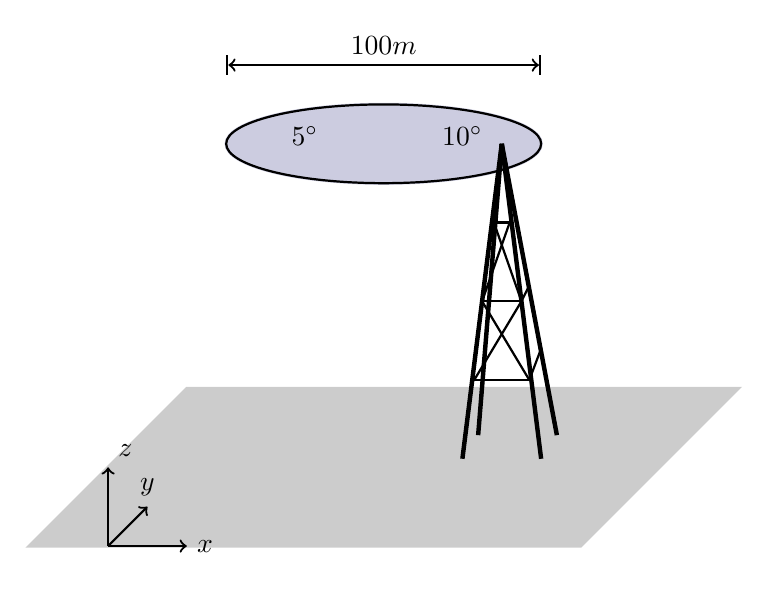
\begin{tikzpicture}
			% ground
			\begin{scope}[yshift=-60,yslant=0,xslant=1]
				\filldraw[black!20,very thick] (-7,1) rectangle (0,3);
				\draw[->, thick] (-6, 1) -- (-5, 1) node[right] {\( x \)};
				\draw[->, thick] (-6, 1) -- (-6, 1.5) node[above] {\( y \)};
				\draw[->, thick] (-6, 1) -- (-7, 2) node[above right] {\( z \)};
			\end{scope}
			% eddy
			\filldraw[black!60!blue!20, very thick] (-1.5, 4) ellipse [x radius=2, y radius=0.5];
			\draw[thick] (-1.5, 4) ellipse [x radius=2, y radius=0.5];
			\node at (-2.5,4.1) {$5^\circ$};
			\node at (-0.5,4.1) {$10^\circ$};
			\draw[|<->|, thick] (-3.5, 5) -- (0.5, 5) node[midway, above] {$100m$};
			% Slant lines
			\draw[ultra thick] (-0.5, 0) -- (0, 4);
			\draw[ultra thick] (-0.3, 0.3) -- (0, 4);
			\draw[ultra thick] (0.5, 0) -- (0, 4);
			\draw[ultra thick] (0.7, 0.3) -- (0, 4);
			% Horizontal lines
			\draw[thick] (-0.35, 1) -- (0.35, 1);
			\draw[thick] (-0.25, 2) -- (0.25, 2);
			\draw[thick] (-0.10, 3) -- (0.10, 3);
			\draw[thick] (0.35, 1) -- (0.5, 1.4);
			\draw[thick] (0.25, 2) -- (0.35, 2.2);
			% Crosses at intersections
			\draw[thick] (-0.35, 1) -- (0.25, 2);
			\draw[thick] (-0.25, 2) -- (0.35, 1);
			\draw[thick] (-0.10, 3) -- (0.25, 2);
			\draw[thick] (-0.25, 2) -- (0.10, 3);
		\end{tikzpicture}
	}
	\renewcommand{\thefigure}{2.1}
	\caption{Eddy propagation}
\end{figure}

\begin{figure}[h!]
	\centering
	\resizebox{0.45\textwidth}{!}{
		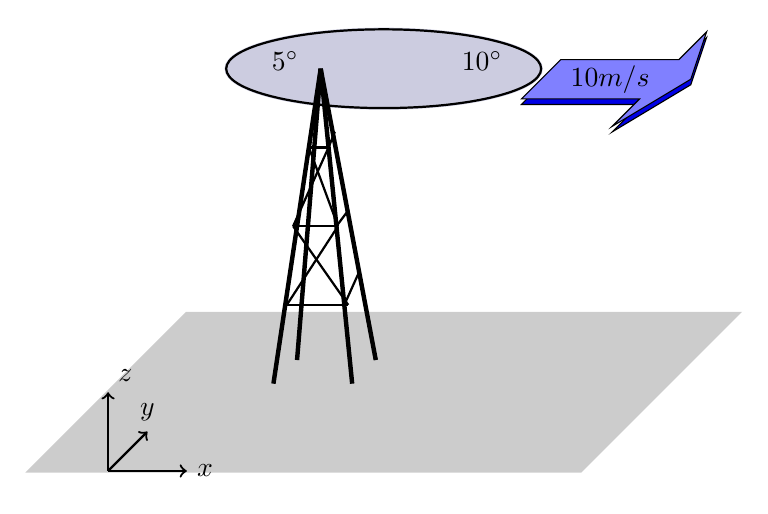
\begin{tikzpicture}
			% ground
			\begin{scope}[yshift=-60,yslant=0,xslant=1]
				\filldraw[black!20,very thick] (-5,1) rectangle (2,3);
				\draw[->, thick] (-4, 1) -- (-3, 1) node[right] {\( x \)};
				\draw[->, thick] (-4, 1) -- (-4, 1.5) node[above] {\( y \)};
				\draw[->, thick] (-4, 1) -- (-5, 2) node[above right] {\( z \)};
			\end{scope}
			\begin{scope}[yshift=108,yslant=0,xslant=1]
				\draw[fill=blue!90!black] (2.5,0.25) --  (4,0.25) coordinate (f1)
				-- (4,0.6) coordinate (f2) -- (4.4,0) coordinate (f3)
				-- (4,-0.6) coordinate (f4) -- (4,-0.25) coordinate (f5)
				-- (2.5,-0.25) coordinate (f6) -- cycle;
			\end{scope}
			\begin{scope}[yshift=110,yslant=0,xslant=1]
				\draw[fill=blue!50] (2.5,0.25) --  (4,0.25) coordinate (f1)
				-- (4,0.6) coordinate (f2) -- (4.4,0) coordinate (f3)
				-- (4,-0.6) coordinate (f4) -- (4,-0.25) coordinate (f5)
				-- (2.5,-0.25) coordinate (f6) -- cycle;
				\path (2, 0) -- (4, 0) node[pos=1, font=\sffamily, anchor=east]{$10m/s$};
			\end{scope}
			% eddy
			\filldraw[black!60!blue!20, very thick] (0.5, 4) ellipse [x radius=2, y radius=0.5];
			\draw[thick] (0.5, 4) ellipse [x radius=2, y radius=0.5];
			\node at (-0.75,4.1) {$5^\circ$};
			\node at (1.75,4.1) {$10^\circ$};
			% Slant lines
			\draw[ultra thick] (-0.9, 0) -- (-0.3, 4);
			\draw[ultra thick] (-0.6, 0.3) -- (-0.3, 4);
			\draw[ultra thick] (0.1, 0) -- (-0.3, 4);
			\draw[ultra thick] (0.4, 0.3) -- (-0.3, 4);
			% Horizontal lines
			\draw[thick] (-0.73, 1) -- (0.05, 1);
			\draw[thick] (-0.65, 2) -- (-0.08, 2);
			\draw[thick] (-0.45, 3) -- (-0.2, 3);
			\draw[thick] (0, 1) -- (0.18, 1.4);
			\draw[thick] (-0.1, 2) -- (0.05, 2.2);
			\draw[thick] (-0.2, 3) -- (-0.12,3.2);
			% Crosses at intersections
			\draw[thick] (-0.73, 1) -- (-0.08, 2);
			\draw[thick] (-0.65, 2) -- (0.05, 1);
			\draw[thick] (-0.65, 2) -- (-0.2, 3);
			\draw[thick] (-0.45, 3) -- (-0.08, 2);
		\end{tikzpicture}
	}
	\renewcommand{\thefigure}{2.2}
	\caption{Eddy passing by the sensor mounted on tower}
\end{figure}

\begin{align*}
	\frac{\partial T}{\partial x} = 0.05 \text{K/m,} \quad \frac{\partial T}{\partial t} = -0.5 \text{K/s} \\
	\underbrace{\cancel{\frac{D T}{D t}}}_{\substack{\text{Total derivative = 0}                           \\ \text{ (Taylor's hypothesis)}}} =\underbrace{\frac{\partial T}{\partial t}}_{\text{Local derivative}} + \underbrace{u\frac{\partial T}{\partial x}}_{\text{Advective term}} \tag{2.1} \label{eq:totoalderivative}
\end{align*}

\subsection{Virtual Potential Temperature}
Virtual potential temperature:
\begin{align*}
	\theta_v = \theta(1+0.61r) \tag{2.2} \label{eq:virtualpotentialtemp}
\end{align*}
Virtual temperature:
\begin{align*}
	T_v = T(1+0.61r) \tag{2.3} \label{eq:virtualtemp}
\end{align*}

\begin{figure}[ht!]
	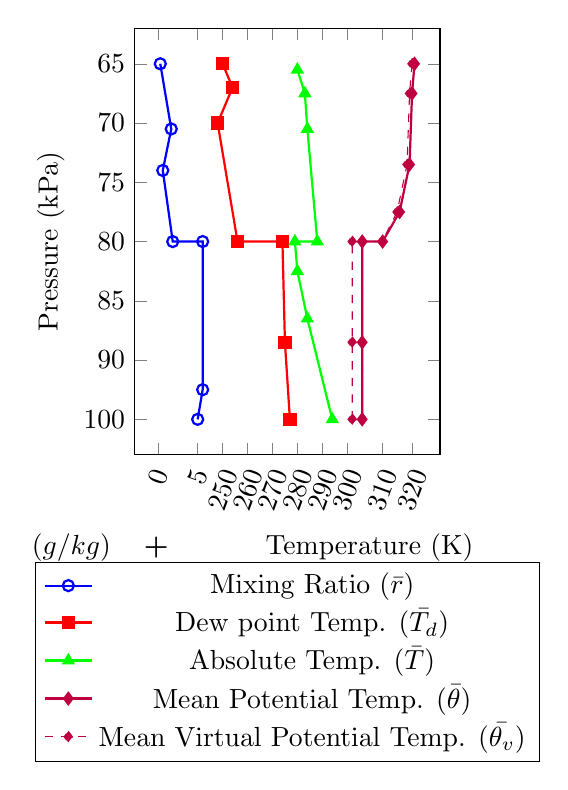
\begin{tikzpicture}
		\centering
		\begin{axis}[
				%axis lines=middle,
				xlabel={\hspace{-1cm} ($g/kg$) \hspace{0.3cm}$\textbf{+}$ \hspace{1cm} Temperature (K)},
				ylabel={Pressure (kPa)},
				legend style={at={(0.5,-0.25)}, anchor=north},
				width=0.45\textwidth, height=7cm,
				xtick=      {0.2, 1, 1.5, 2,    2.5, 3,   3.5,  4,   4.7,   5.3},
				xticklabels={0,   5, 250, 260,  270, 280, 290,  300, 310, 320},
				ytick=      {0,   1,  2,  3,  4,  5,  6},
				yticklabels={100, 90, 85, 80, 75, 70, 65},
				xticklabel style={rotate=70},
				% yticklabel style={rotate=0}
			]
			\addplot[mark=o, blue, thick] coordinates {
					(1,0) (1.1,0.5) (1.1,3) (0.5,3) (0.3,4.2) (0.47,4.9) (0.25,6)
				};
			\addlegendentry{Mixing Ratio ($\bar{r}$)}

			\addplot[mark=square*, red, thick] coordinates {
					(2.85,0) (2.75,1.3) (2.7,3)  (1.8,3) (1.4,5) (1.7,5.6) (1.5,6)
				};
			\addlegendentry{Dew point Temp. (${\bar{T_d}}$)}

			\addplot[mark=triangle*, green, thick] coordinates {
					(3.7,0) (3.2,1.7) (3,2.5) (2.95,3) (3.4,3) (3.2,4.9) (3.15,5.5) (3.0,5.9)
				};
			\addlegendentry{Absolute Temp. (${\bar{T}}$)}

			\addplot[mark=diamond*, purple, thick] coordinates {
					(4.3,0) (4.3,1.3) (4.3,3) (4.71,3) (5.05,3.5) (5.25,4.3) (5.3,5.5) (5.35,6)
				};
			\addlegendentry{Mean Potential Temp. (${\bar{\theta}}$)}

			\addplot[mark=diamond*, purple, dashed] coordinates {
					(4.1,0) (4.1,1.3) (4.1,3) (4.7,3) (5,3.5) (5.2,4.3) (5.25,5.5) (5.3,6)
				};
			\addlegendentry{Mean Virtual Potential Temp. (${\bar{\theta_v}}$)}
		\end{axis}
	\end{tikzpicture}
	\renewcommand{\thefigure}{2.3}
	\caption{Pressure v/s Termperature}
\end{figure}

\begin{question}{}
	Given 25$^\circ$C termperature, mixing ratio $\bar{r}$ is 20$g/kg$, measured Pressurere at 900$hPa$, find virtual potential temperature.
\end{question}
\begin{answer}{}
	Solution:\begin{align*}
		\theta            & = T \times \Big(\frac{1000}{P}\Big)^{0.286}      \\
		                  & = 298 \times \Big(\frac{1000}{900}\Big)^{0.286}  \\
		                  & = 332.222 K                                      \\
		\theta_v          & = \theta \times \big(1 + 0.61r \big)             \\
		                  & = 332.22 \times \big(1 + 0.61 \times 0.025 \big) \\
		                  & = 336.273 K                                      \\
		\theta_v - \theta & \approx 4.05 K
	\end{align*}
\end{answer}

\subsection{Boundary Layer Depth and Structure}
\begin{itemize}[noitemsep]
	\item Mixed layer
	\item Residual layer
	\item Stable Boundary layer
	\item Capping Inversion
	\item Nauturnal Boundary layer
\end{itemize}

\begin{figure*}[t!]
	\centering
	\resizebox{0.9\textwidth}{!}{
		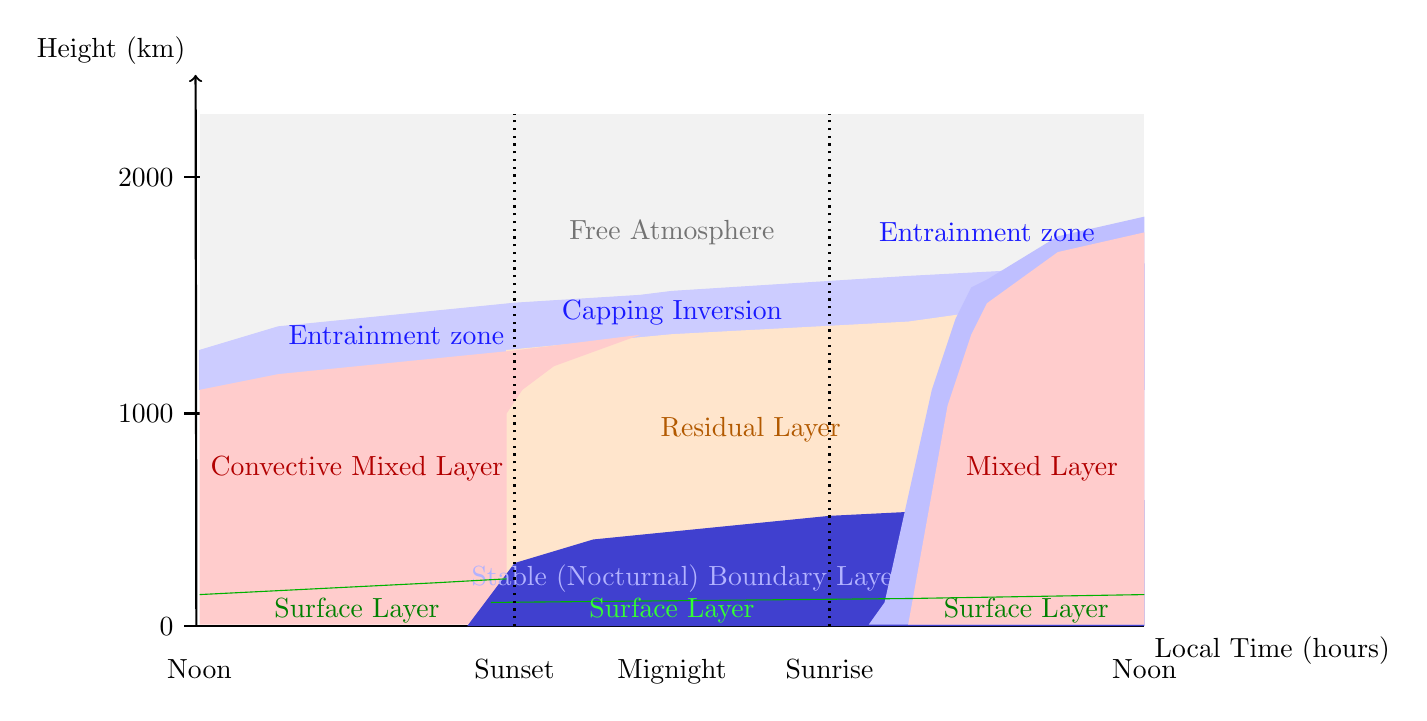
\begin{tikzpicture}
			% Axes
			\draw[thick,-] (-0.04,0) -- (12,0) node[below right] {Local Time (hours)};
			\draw[thick,->] (-0.04,0) -- (-0.05,7) node[above left] {Height (km)};
			% Time ticks
			% \foreach \x in {0,1,...,12} {
			% 		\draw[thick] (\x,0) -- (\x,-0.2) node[below] {\x};
			% 	}
			% Height ticks
			\foreach \y/\label in {0/0, 2.7/1000, 5.7/2000} {
					\draw[thick] (0,\y) -- (-0.2,\y) node[left] {\label};
				}
			% Free Atmosphere
			\fill[gray!10] (0,3) -- (12,3) -- (12,6.5) -- (0,6.5) -- cycle;
			\node[gray!90!black] at (6,5) {Free Atmosphere};
			% Capping Inversion
			\filldraw[blue!20] (0,3) -- (0,3.5) -- (1,3.8) -- (2,3.9) -- (4,4.1) -- (5.6,4.2) -- (6,4.25) -- (9,4.44) -- (12,4.6) -- (12, 3);
			\node[blue!90, above] at (6,3.7) {Capping Inversion};
			% % Entrainment Zone
			% \fill[cyan!30, opacity=0.5] (3,3) -- (6,3.5) -- (9,3.3) -- (12,3.1) -- (12,2.8) -- (9,2.8) -- (6,3) -- (3,3) -- cycle;
			% \node[cyan!70!black] at (6,3.3) {Entrainment Zone};
			% Residual Layer
			\filldraw[orange!20] (3.9,0.02) -- (3.9,3.5) -- (6, 3.7) -- (9,3.86) -- (10,4) -- (9.8, 3.7) -- (9.5, 2.8) -- (9,0.2);
			\node[orange!70!black] at (7,2.5) {Residual Layer};
			% Convective Mixed Layer
			\fill[red!20] (0,0.02) -- (0,3) -- (1,3.2) -- (2,3.3) -- (4,3.5) -- (5.6,3.7) -- (4.5, 3.3) -- (4.1,3) -- (3.9,2.7) -- (3.9,0.02) -- cycle;
			\node[red!70!black] at (2,2) {Convective Mixed Layer};
			% Stable Boundary Layer (Nocturnal)
			\fill[blue!75!black!75] (3.4,0) -- (4,0.8) -- (5,1.1) -- (8,1.4) -- (12,1.6) -- (12,0) -- cycle;
			\node[blue!30] at (6.2,0.6) {Stable (Nocturnal) Boundary Layer};
			% Entrainment Zone
			\fill[blue!25] (8.5,0.02) -- (8.7, 0.3) -- (9.3,3) -- (9.6,3.9) -- (9.8,4.3) -- (10, 4.4) -- (10.9,4.95) -- (12, 5.2) -- (12, 0.02) -- cycle;
			\node[blue!90] at (10,5) {Entrainment zone};
			\node[blue!90] at (2.5,3.7) {Entrainment zone};
			% Mixed Layer
			\fill[red!20] (10,3.9) -- (9.8,3.7) -- (9.5,2.8) -- (9,0.02) -- (12, 0.02) -- (12, 5) -- (10.9,4.75) -- (10, 4.1) -- (9.8,3.7) -- cycle;
			\node[red!70!black] at (10.7,2) {Mixed Layer};
			% Surface Layer
			\draw[green!70!black] (0,0.4) -- (3,0.55) -- (3.9,0.6);
			\draw[green!70!black] (3.7,0.3) -- (9,0.35) -- (12,0.4);
			\node[green!50!black] at (2,0.2) {Surface Layer};
			\node[green!80] at (6,0.2) {Surface Layer};
			\node[green!50!black] at (10.5,0.2) {Surface Layer};
			% Sunrise and Sunset lines
			\draw[dotted, thick] (4,0) -- (4,6.5);
			\draw[dotted, thick] (8,0) -- (8,6.5);
			% Day/Night Labels
			\node[below] at (0,-0.3) {Noon};
			\node[below] at (4,-0.3) {Sunset};
			\node[below] at (6,-0.3) {Mignight};
			\node[below] at (8,-0.3) {Sunrise};
			\node[below] at (12,-0.3) {Noon};
		\end{tikzpicture}
	}
	\label{fig:boundary_layer}
	\renewcommand{\thefigure}{2.4}
	\caption{Height vs Local Time Diagram of Atmospheric Boundary Layers.}
\end{figure*}

\clearpage
\section{Lecture 3 16/01/2025}

\textbf{Ocean:} Variations are minimal, with only 10\% changes observed over 1000 km. Significant variations occur primarily during weather phenomena.

\textbf{Land:} Day-to-day and diurnal variations are prominent, with distinct boundary layer structures:

\vspace{-0.25cm}
\begin{enumerate}[noitemsep]
	\item \textbf{Convective Mixed Layer:} Thermodynamically unstable with intense vertical mixing.
	\item \textbf{Residual Layer:} Neutral stratification with turbulence of equal intensity in all directions.
	\item \textbf{Stable Boundary Layer (Nocturnal B.L.):}
	      \begin{itemize}[noitemsep, topsep=0pt, partopsep=0pt]
		      \item Neutral stratification with nocturnal jets (~30 m/s, ~200 m width).
		      \item Sporadic turbulence and internal gravity waves transporting air parcels vertically.
	      \end{itemize}
	\item \textbf{Capping Inversion:} Found at altitudes between 1.5–3 km, acting as a barrier to upward mixing.
	\item \textbf{Entrainment Zone:} Transition region from stable to unstable conditions, facilitating energy and mass exchange.
\end{enumerate}

\subsection{Stability and Plume Behaviour}
\begin{enumerate}[noitemsep]
	\item \textbf{Looping plumes:} Occur in highly unstable conditions, usually during the day, when strong surface heating causes warm air to rise and interact turbulently with cooler air. This leads to an oscillatory motion that disperses pollutants in multiple directions, often seen in arid regions.
	\item \textbf{Fanning plumes:} Form in stable conditions, typically at night, when surface cooling creates temperature inversions. The plume spreads horizontally, concentrating pollutants close to the surface, which can impact air quality in urban or industrial areas.
	\item \textbf{Coning plumes:} Develop under neutral conditions, where vertical and horizontal mixing is balanced. The plume takes a cone-like shape, often observed on overcast days or in the early morning and evening, with moderate turbulence.
	\item \textbf{Lofting plumes:} Occur when the atmosphere is stable near the ground but unstable above. Pollutants rise and disperse above the stable layer, reducing ground-level pollution and minimizing surface concentrations.
	\item \textbf{Fumigation plumes:} Happen when pollutants are trapped in a stable layer and then forced downward due to rising turbulence. This leads to high concentrations at the surface, posing risks to air quality, especially in industrial areas.
\end{enumerate}

\freeyellownote{0}{-400}{FIGURE for each to be added later.}

\subsection{Importance of Boundary Layer}
The boundary layer plays a critical role in regulating interactions between the Earth's surface and the atmosphere. Its study is important in various fields, including:

\begin{enumerate}[noitemsep]
	\item \textbf{Agricultural meteorology:} Understanding microclimates within the boundary layer aids in crop management, irrigation planning, and predicting the effects of extreme weather on agriculture.
	\item \textbf{Air pollution meteorology:} Dispersion and concentration of pollutants are governed by boundary layer processes, making it crucial for air quality monitoring and pollution control strategies.
	\item \textbf{Cloud nuclei meteorology:} The boundary layer provides a reservoir of aerosols and moisture that act as cloud condensation nuclei, influencing cloud formation, precipitation, and local weather patterns.
	\item \textbf{Thunderstorms and hurricanes physics:} The exchange of heat, moisture, and momentum in the boundary layer drives the development and intensity of thunderstorms and hurricanes, making it essential for improving weather prediction models.
	\item \textbf{Urban meteorology:} The boundary layer's interactions with urban landscapes affect local climate, energy balance, and pollutant dispersion, aiding in city planning and sustainability efforts.
	\item \textbf{Renewable energy:} Wind energy potential and efficiency are heavily dependent on boundary layer dynamics, which dictate wind speed profiles and turbulence levels near the surface.
\end{enumerate}

\begin{table}[ht!]
	\centering
	\begin{tabular}{|p{1.6cm}|p{3cm}|p{3cm}|}
		\hline
		\rowcolor{blue!20} \textbf{Property}            & \textbf{Boundary Layer}                & \textbf{Free Atmosphere}                \\
		\hline
		\cellcolor{blue!10} \textbf{Turbulence}         & Almost continuously turbulent          & Sporadic, CAT, turbulence within clouds \\
		\hline
		\cellcolor{blue!10} \textbf{Friction}           & Strong drag due to surface interaction & Small viscous dissipation               \\
		\hline
		\cellcolor{blue!10} \textbf{Dispersion}         & Rapid turbulent mixing                 & Small molecular diffusion               \\
		\hline
		\cellcolor{blue!10} \textbf{Winds}              & Near logarithmic profile               & Geostrophic winds                       \\
		\hline
		\cellcolor{blue!10} \textbf{Vertical Transport} & Turbulent vertical motion              & Horizontal transport by mean wind       \\
		\hline
		\cellcolor{blue!10} \textbf{Thickness}          & 100m - 3km (variable)                  & 8-16km (less variable)                  \\
		\hline
	\end{tabular}
	\caption{Comparison of Boundary Layer and Free Atmosphere Properties}
	\label{tab:boundary_free}
\end{table}

\clearpage

\section{Lecture 4 23/01/2025}
\subsection{Statistical Tools Required For Turbulence}

Turbulence is characteristiced by randomness.
\begin{align*}
	U & = \overline{u} + u' \\
	V & = \overline{v} + v' \\
	W & = \overline{w} + w' \\
	C & = \overline{c} + c'
\end{align*}

\subsubsection{Mean}
\begin{align*}
	\overline{A} & = \frac{1}{N}\sum^N_{i=1}A(i,s)   \\
	\overline{A} & = \frac{1}{T}\int^T_{t=0}A(t,s)dt
\end{align*}

\subsubsection{Rules for averaging}
If $A$ and $B$ are variables dependent on time, then:
\begin{align*}
	\overline{A + B}                & = \overline{A} + \overline{B}, \\
	\overline{\overline{A}}         & = A,                           \\
	\overline{\overline{A} \cdot B} & = \overline{A \cdot B},        \\
	\overline{\frac{dA}{dt}}        & = \frac{d\overline{A}}{dt}.
\end{align*}

\textbf{Reynold's averaging rule}
\begin{align*}
	\overline{\overline{A}}         & = \overline{\overline{A}+a'} = \overline{A}, \text{since } \overline{a'}=0                      \\
	\overline{\overline{A \cdot B}} & = \overline{(\overline{A}+a')(\overline{B}+b')} = \overline{A}\overline{B} + \overline{(a'b')}, \\
	\overline{(a'b')}               & \neq  \overline{a'}\overline{b'}                                                                \\
	\overline{a'^2}                 & \neq 0                                                                                          \\
	\overline{b'^2}                 & \neq 0
\end{align*}

\subsubsection{Variance}
\begin{align*}
	\sigma_A^2 & = \frac{1}{N} \sum^N_{i=1}(A_i-\overline{A})^2 = \overline{a'^2}
\end{align*}

\subsubsection{Standard deviation}
\begin{align*}
	\sigma_A & = \sqrt{\frac{1}{N} \sum^N_{i=1}(A_i-\overline{A})^2} = \Big(\overline{a'^2}\Big)^2
\end{align*}

\subsubsection{Covariance}
\begin{align*}
	\sigma_{A,B} & = \frac{1}{N} \sum_{i=1}^N (A_i - \overline{A})(B_i - \overline{B}) = \overline{a'b'}.
\end{align*}

\subsubsection{Correlation}
\begin{align*}
	\gamma_{A,B} & = \frac{\overline{a'b'}}{\sigma_A\sigma_B}
\end{align*}

Mean Kinetic Energy (MKE) = $\frac{1}{2}(\overline{u}^2 + \overline{v}^2 +\overline{w}^2)$ \\
Turbulent Kinetic Energy (TKE) = $\frac{1}{2}(\overline{u'}^2 + \overline{v'}^2 +\overline{w'}^2)$

\begin{question}{}
	Suppose we erect instruments with an anemometer to measure \(u\) and \(w\) components, recording wind speeds every 6 seconds for a minute, resulting in the following 10 points of wind observations shown in Table~\ref{tab:wind-observations}. Calculate the mean, variance, and standard deviation for each component. Also, find the covariance and correlation between them.
\end{question}
\begin{table}[h!]
	\centering
	\begin{tabular}[c]{|>{\columncolor{black!30}}l|l|l|l|l|l|l|l|l|l|l|}
		\hline
		\textbf{u (m/s)} & 5 & 6  & 5 & 4 & 7  & 5 & 3 & 5  & 4 & 6  \\
		\hline
		\textbf{w (m/s)} & 0 & -1 & 1 & 0 & -2 & 1 & 2 & -1 & 1 & -1 \\
		\hline
	\end{tabular}
	\caption{Wind observations for \(u\) and \(w\) components.}
	\label{tab:wind-observations}
\end{table}
\begin{answer}{}
	Solution:\begin{align*}
		\overline{u}                   & = 5, \qquad \overline{v} = 0              \\
		\sigma^2_U                     & = 1.2, \qquad \sigma^2_W = 1.1            \\
		\sigma_U                       & = \sqrt{1.2}, \quad \sigma_W = \sqrt{1.1} \\
		\sigma_{U,W} = \overline{u'w'} & = -1.1, \quad \gamma_{U,W} =
	\end{align*}
\end{answer}

\clearpage

\section{Lecture 5 24/01/2025}
\subsection{Fluxes}
Mass, Heat, Moisture, Momentum, Pollutent, etc.

\begin{table}[h!]
	\begin{center}
		\begin{tabular}[c]{|l|l|}
			\hline
			\multicolumn{1}{|>{\columncolor{blue!20}}c|}{\textbf{Quantity}} &
			\multicolumn{1}{>{\columncolor{blue!20}}c|}{\textbf{Unit}}                                     \\
			\hline
			Mass                                                            & $kg_{\text{air}}/m^2s$       \\
			Heat                                                            & $J/m^2s$                     \\
			Moisture                                                        & $kg_{\text{wv}}/m^2s$        \\
			Momentum                                                        & $kgms^{-1}/m^2s$             \\
			Pollutant                                                       & $kg_{\text{pollutant}}/m^2s$ \\
			\hline
		\end{tabular}
	\end{center}
\end{table}

\subsection{Kinematic Flux}
\textbf{Note:} We asssume atmoshpere to be of constant density ($\rho_{\text{air}}$).

\begin{table}[h!]
	\begin{center}
		\begin{tabular}[c]{|l|l|l|}
			\hline
			\multicolumn{1}{|>{\columncolor{blue!20}}c|}{\textbf{Flux Quantity}} &
			\multicolumn{1}{>{\columncolor{blue!20}}c|}{\textbf{Formula}}        &
			\multicolumn{1}{>{\columncolor{blue!20}}c|}{\textbf{Unit}}                                                                                    \\
			\hline
			Mass flux                                                            & $\frac{\text{mass}}{\rho_{\text{air}}}$ & $kg_{\text{air}}/m^2s$       \\
			Heat flux                                                            & $\frac{\text{heat}}{\rho C_p}$          & $J/m^2s$                     \\
			Moisture flux                                                        & -                                       & $kg_{\text{wv}}/m^2s$        \\
			Momentum flux                                                        & -                                       & $kgms^{-1}/m^2s$             \\
			Pollutant flux                                                       & -                                       & $kg_{\text{pollutant}}/m^2s$ \\
			\hline
		\end{tabular}
	\end{center}
\end{table}

Examples:-
\begin{align*}
	\text{Veritcal advective heat flux}    & = \overline{w}\overline{\theta} \\
	\text{x-direction advective heat flux} & = \overline{u}\overline{\theta} \\
	\text{x-direction moisture flux}       & = \overline{u}\overline{q}      \\
	\text{Veritcal eddy heat flux}         & = \overline{w\theta}            \\
	\text{x-direction eddy flux}           & = \overline{uq}
\end{align*}

x-direction solar flux = $\Big(\frac{1/4S_0}{c_p\rho}\Big)$ = 0.2773 Km/s

\subsection{Eddy Flux}
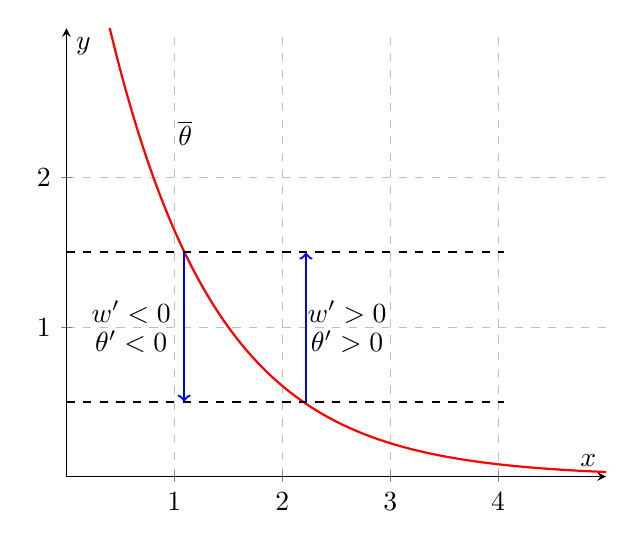
\begin{tikzpicture}
	\begin{axis}[
			axis lines=middle,
			xlabel={$x$},
			ylabel={$y$},
			xmin=0, xmax=5,
			ymin=0, ymax=3,
			domain=0:5,
			samples=100,
			xtick={0,1,2,3,4},
			ytick={-2,-1,0,1,2},
			grid=major,
			grid style={dashed,gray!50},
		]
		\addplot[red, thick] {exp(-x+1.5)};

		\node at (1.1,2.3) {$\overline\theta$};
		\node at (0.6,1.1) {$w'<0$};
		\node at (0.6,0.9) {$\theta'<0$};
		\node at (2.6,1.1) {$w'>0$};
		\node at (2.6,0.9) {$\theta'>0$};

		\draw[black, dashed, thick] (0,1.5) -- (4.05,1.5);
		\draw[black, dashed, thick] (0,0.5) -- (4.05,0.5);

		\draw[->, blue, thick] (axis cs: 1.09, 1.5) -- ++(0, -1);
		\draw[<-, blue, thick] (axis cs: 2.22, 1.5) -- ++(0, -1);
	\end{axis}
\end{tikzpicture}

\begin{align*}
	\Delta w'                    & = 0 \\
	\Delta(\overline{w'\theta'}) & > 0
\end{align*}

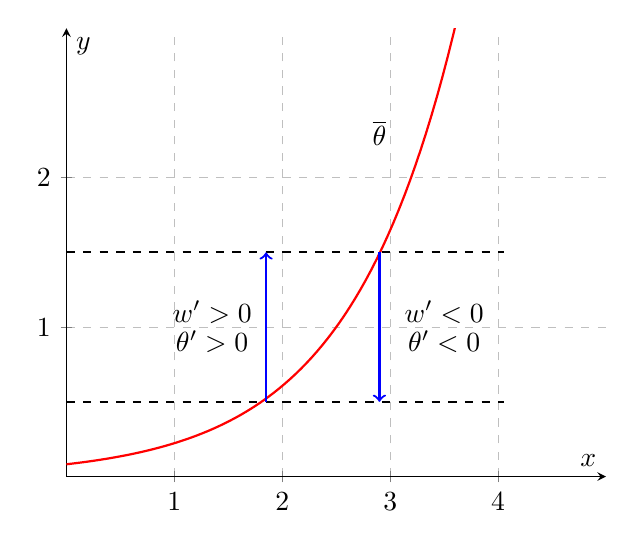
\begin{tikzpicture}
	\begin{axis}[
			axis lines=middle,
			xlabel={$x$},
			ylabel={$y$},
			xmin=0, xmax=5,
			ymin=0, ymax=3,
			domain=0:5,
			samples=100,
			xtick={0,1,2,3,4},
			ytick={-2,-1,0,1,2},
			grid=major,
			grid style={dashed,gray!50},
		]
		\addplot[red, thick] {exp(x-2.5)};

		\node at (2.9,2.3) {$\overline\theta$};
		\node at (3.5,1.1) {$w'<0$};
		\node at (3.5,0.9) {$\theta'<0$};
		\node at (1.35,1.1) {$w'>0$};
		\node at (1.35,0.9) {$\theta'>0$};

		\draw[black, dashed, thick] (0,1.5) -- (4.05,1.5);
		\draw[black, dashed, thick] (0,0.5) -- (4.05,0.5);

		\draw[->, blue, thick] (axis cs: 2.9, 1.5) -- ++(0, -1);
		\draw[<-, blue, thick] (axis cs: 1.85, 1.5) -- ++(0, -1);
	\end{axis}
\end{tikzpicture}

\begin{align*}
	\Delta w'                    & = 0 \\
	\Delta(\overline{w'\theta'}) & < 0
\end{align*}

\subsection{Stress}
Force tending to produce deformation in a body is called \textbf{Stress}.

\begin{center}
	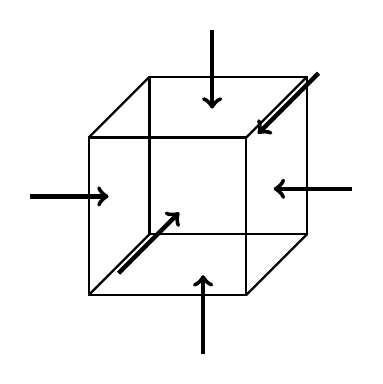
\begin{tikzpicture}[scale=1]
		% Draw cube
		\draw[thick] (2,2,2) -- (4,2,2) -- (4,4,2) -- (2,4,2) -- cycle; % Bottom face
		\draw[thick] (2,2,4) -- (4,2,4) -- (4,4,4) -- (2,4,4) -- cycle; % Top face
		\draw[thick] (2,2,2) -- (2,2,4); % Vertical edges
		\draw[thick] (4,2,2) -- (4,2,4);
		\draw[thick] (4,4,2) -- (4,4,4);
		\draw[thick] (2,4,2) -- (2,4,4);

		% Shade the upper and lower faces
		% \fill[gray!30,opacity=0.7] (2,2,4) -- (4,2,4) -- (4,2,2) -- (2,2,2) -- cycle; % Bottom face
		% \fill[gray!50,opacity=0.7] (2,4,4) -- (4,4,4) -- (4,4,2) -- (2,4,2) -- cycle; % Top face

		\draw[->, ultra thick] (2.7,4.5,1.75) -- (2.7,3.5,1.75);
		\draw[->, ultra thick] (2.2,0,0.75) -- (2.2,1,0.75);
		\draw[->, ultra thick] (0,2,0.75) -- (1,2,0.75);
		\draw[->, ultra thick] (4,2,0.5) -- (3,2,0.5);
		\draw[->, ultra thick] (1.8,1.7,2.5) -- (1.8,1.7,0.5);
		\draw[->, ultra thick] (2.8,2.7,-1.5) -- (2.8,2.7,0.5);
	\end{tikzpicture}
\end{center}

\subsubsection{Reynold's stress}

\begin{center}
	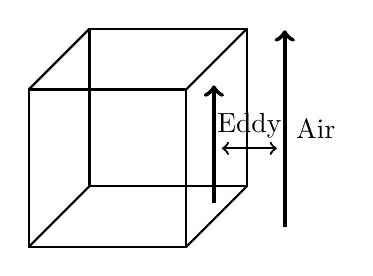
\begin{tikzpicture}[scale=1]
		% Draw cube
		\draw[thick] (2,2,2) -- (4,2,2) -- (4,4,2) -- (2,4,2) -- cycle; % Bottom face
		\draw[thick] (2,2,4) -- (4,2,4) -- (4,4,4) -- (2,4,4) -- cycle; % Top face
		\draw[thick] (2,2,2) -- (2,2,4); % Vertical edges
		\draw[thick] (4,2,2) -- (4,2,4);
		\draw[thick] (4,4,2) -- (4,4,4);
		\draw[thick] (2,4,2) -- (2,4,4);

		% Shade the upper and lower faces
		% \fill[gray!30,opacity=0.7] (2,2,4) -- (4,2,4) -- (4,2,2) -- (2,2,2) -- cycle; % Bottom face
		% \fill[gray!50,opacity=0.7] (2,4,4) -- (4,4,4) -- (4,4,2) -- (2,4,2) -- cycle; % Top face

		\draw[->, ultra thick] (4,1,0.75) -- (4,3.5,0.75) node[midway, right] {\text{Air}};
		\draw[<->, thick] (3.2,2,0.75) -- (3.9,2,0.75) node[midway, above] {\text{Eddy}};
		\draw[->, ultra thick] (3.1,1.3,0.75) -- (3.1,2.8,0.75);
	\end{tikzpicture}

	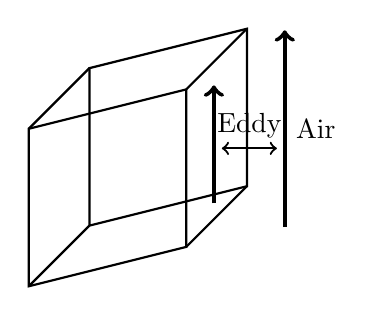
\begin{tikzpicture}[scale=1]
		% Draw cube
		\draw[thick] (2,2,2) -- (4,2.5,2) -- (4,4.5,2) -- (2,4,2) -- cycle; % Bottom face
		\draw[thick] (2,2,4) -- (4,2.5,4) -- (4,4.5,4) -- (2,4,4) -- cycle; % Top face
		\draw[thick] (2,2,2) -- (2,2,4); % Vertical edges
		\draw[thick] (4,2.5,2) -- (4,2.5,4);
		\draw[thick] (4,4.5,2) -- (4,4.5,4);
		\draw[thick] (2,4,2) -- (2,4,4);

		\draw[->, ultra thick] (4,1.5,0.75) -- (4,4,0.75) node[midway, right] {\text{Air}};
		\draw[<->, thick] (3.2,2.5,0.75) -- (3.9,2.5,0.75) node[midway, above] {\text{Eddy}};
		\draw[->, ultra thick] (3.1,1.8,0.75) -- (3.1,3.3,0.75);
	\end{tikzpicture}
\end{center}

\clearpage

\section{Lecture 6 29/01/2025}
\subsection{Summation Notation}
\textbf{Definition:} Integer variables \( m, n, \) and \( q \) can take values \( 1,2,3 \). Then:
\vspace{-5pt}
\begin{itemize}[noitemsep]
	\item \( A_m \) is a velocity vector.
	\item \( X_m \) represents distance.
\end{itemize}

where, \vspace{-10pt}
\begin{align*}
	m & = 1,2,3, \\
	n & = 1,2,3, \\
	q & = 1,2,3.
\end{align*}

Hence, \vspace{-10pt}
\begin{align*}
	A_1 & = u, & A_2 & = v, & A_3 & = w, \\
	X_1 & = x, & X_2 & = y, & X_3 & = z.
\end{align*}

\subsection{Unit vector}
Unit vector is represented by $\delta_m$,

where, \vspace{-5pt}
\begin{align*}
	\delta_1 & = \hat{i}, \\
	\delta_2 & = \hat{j}, \\
	\delta_3 & = \hat{k}
\end{align*}

\subsection{Kronecker Delta}
Kronecker Delta is represented by $\delta_{mn}$, such that,

\begin{align*}
	\delta_{mn} =
	\begin{cases}
		1, & \text{for } m = n,   \\
		0, & \text{for } m \neq n
	\end{cases}
\end{align*}

\subsection{Alternating Unit Tensor}
Alternating Unit Tensor is represented by $\epsilon_{mn}$, such that,

\begin{align*}
	\delta_{mn} =
	\begin{cases}
		+1, & \text{for } mnq = 123,231,312          \\
		-1, & \text{for } mnq = 321,132,213          \\
		0,  & \text{for any 2 or more indices alike}
	\end{cases}
\end{align*}

\subsection{Rules For Summation Notation}
\subsubsection*{Rule I:}
Wherever two identical appear same in one term, it is implied that there is a sum of that term over each value of repreated index.

For example:

1. \vspace{-15pt}
\begin{align*}
	A_n\frac{\partial B_m}{\partial X_n} & = A_1\frac{\partial B_m}{\partial X_1} + A_2\frac{\partial B_m}{\partial X_2} + A_3\frac{\partial B_m}{\partial X_3} \\
	                                     & = u\frac{\partial B_m}{\partial x} + v\frac{\partial B_m}{\partial y} + w\frac{\partial B_m}{\partial z}
\end{align*}

2. \vspace{-20pt}
\begin{align*}
	\delta_{2n}A_n & = \delta_{21}A_1 + \delta_{22}A_3 + \delta_{23}A_3 \\
	               & = A_2                                              \\
	               & = v
\end{align*}

\subsubsection*{Rule II:}
Wherever one index appear unsummed in one term, then the same index appear unsummed in all 3 terms in that equation. Hence that equation effectively represents 3 equations for each value of unsummed index.

\vspace{-10pt}
\begin{align*}
	A_m & = B_m + \delta_{mn}C_n             \\
	A_1 & = B_1 + \delta_{1n}C_n = B_1 + C_1 \\
	A_2 & = B_2 + \delta_{2n}C_n = B_2 + C_2 \\
	A_2 & = B_3 + \delta_{3n}C_n = B_3 + C_3
\end{align*}

For example:

1. \vspace{-17pt}
\begin{align*}
	\frac{\partial A_m}{\partial t} + B_n\frac{\partial A_m}{\partial X_n} = & -\delta_{m3}g + f\epsilon_{mn3}B_n \\ & -\frac{1}{\rho}\frac{\partial P}{\partial X_m} + \frac{1}{\rho}\left[\frac{\tau_{mn}}{\partial X_n}\right]
\end{align*}

Expanding with $n=1,2$ and $3$, we get:
\begin{align*}
	\frac{\partial A_m}{\partial t} & + B_1\frac{\partial A_m}{\partial X_1} + B_2\frac{\partial A_m}{\partial X_2} + B_3\frac{\partial A_m}{\partial X_3} = \\  & -\delta_{m3}g - f[\epsilon_{m13}B_1 + \epsilon_{m23}B_2 + \cancel{\epsilon_{m33}B_3}] \\ & -\frac{1}{\rho}\left[\frac{\partial P}{\partial X_m}\right] + \frac{1}{\rho}\left[\frac{\tau_{m1}}{\partial X_1} + \frac{\tau_{m2}}{\partial X_2} + \frac{\tau_{m3}}{\partial X_3}\right]
\end{align*}

Now expanding with $m=1$, we get following equation:
\begin{align*}
	\frac{\partial A_1}{\partial t} & + B_1\frac{\partial A_1}{\partial X_1} + B_2\frac{\partial A_1}{\partial X_2} + B_3\frac{\partial A_1}{\partial X_3} =                                              \\  & -\cancel{\delta_{13}g} + f[\cancel{\epsilon_{113}B_1} + \epsilon_{123}B_2 + \cancel{\epsilon_{133}B_3}] \\ & -\frac{1}{\rho}\left[\frac{\partial P}{\partial X_1}\right] + \frac{1}{\rho}\left[\frac{\tau_{11}}{\partial X_1} + \frac{\tau_{12}}{\partial X_2} + \frac{\tau_{13}}{\partial X_3}\right] \\
	\frac{\partial u}{\partial t}   & + u\frac{\partial u}{\partial x} + v\frac{\partial u}{\partial y} + w\frac{\partial u}{\partial z} = +fv - \frac{1}{\rho}\left[\frac{\partial P}{\partial x}\right] \\ & + \frac{1}{\rho}\left[\frac{\tau_{xx}}{\partial x} + \frac{\tau_{xy}}{\partial y} + \frac{\tau_{xz}}{\partial z}\right]
\end{align*}

Now expanding with $m=2$, we get following equation:
\begin{align*}
	\frac{\partial A_2}{\partial t} & + B_1\frac{\partial A_2}{\partial X_1} + B_2\frac{\partial A_2}{\partial X_2} + B_3\frac{\partial A_2}{\partial X_3} =                                              \\  & -\cancel{\delta_{23}g} + f[\epsilon_{213}B_1 + \cancel{\epsilon_{223}B_2} + \cancel{\epsilon_{233}B_3}] \\ & -\frac{1}{\rho}\left[\frac{\partial P}{\partial X_2}\right] + \frac{1}{\rho}\left[\frac{\tau_{21}}{\partial X_1} + \frac{\tau_{22}}{\partial X_2} + \frac{\tau_{23}}{\partial X_3}\right] \\
	\frac{\partial v}{\partial t}   & + u\frac{\partial v}{\partial x} + v\frac{\partial v}{\partial y} + w\frac{\partial v}{\partial z} = -fu - \frac{1}{\rho}\left[\frac{\partial P}{\partial y}\right] \\ & + \frac{1}{\rho}\left[\frac{\tau_{yx}}{\partial x} + \frac{\tau_{yy}}{\partial y} + \frac{\tau_{yz}}{\partial z}\right]
\end{align*}

Now expanding with $m=3$, we get following equation:
\begin{align*}
	\frac{\partial A_3}{\partial t} & + B_1\frac{\partial A_3}{\partial X_1} + B_2\frac{\partial A_3}{\partial X_2} + B_3\frac{\partial A_3}{\partial X_3} =                                             \\  & -\delta_{33}g + f[\cancel{\epsilon_{313}}B_1 + \cancel{\epsilon_{323}B_2} + \cancel{\epsilon_{333}B_3}] \\ & -\frac{1}{\rho}\left[\frac{\partial P}{\partial X_3}\right] + \frac{1}{\rho}\left[\frac{\tau_{31}}{\partial X_1} + \frac{\tau_{32}}{\partial X_2} + \frac{\tau_{33}}{\partial X_3}\right] \\
	\frac{\partial w}{\partial t}   & + u\frac{\partial w}{\partial x} + v\frac{\partial w}{\partial y} + w\frac{\partial w}{\partial z} = -g - \frac{1}{\rho}\left[\frac{\partial P}{\partial z}\right] \\ & + \frac{1}{\rho}\left[\frac{\tau_{zx}}{\partial x} + \frac{\tau_{zy}}{\partial y} + \frac{\tau_{zz}}{\partial z}\right]
\end{align*}

\clearpage

\section{Lecture 7 30/01/2025}
\subsection{Governing Equation For Turbulent Flow}
\begin{enumerate}[noitemsep]
	\item Mean variable ($\overline{u}, \overline{v},\overline{w}$).
	\item Flux variable ($\overline{u'w'}, \overline{w'\theta'}$).
	\item Total Kinetic Energy ($\overline{u'^2}, \overline{v'^2},\overline{w'^2}$).
\end{enumerate}

\subsubsection*{Steps:}
\begin{enumerate}[noitemsep]
	\item Identify the basic equations.
	\item Expand the total derivative into local and advective term.
	\item Expand dependent variables into mean and turbulent parts.
	\item Apply Reynold's averaging.
	\item Add continuity equation to put the result in flux part.
\end{enumerate}

\clearpage
\bibliographystyle{plain}
\bibliography{Reference}
\end{document}
